%%%%%%%%%%%%%%%%%%%%%%%%%%%%%%%%%%%%%%%%%%%%%%%%%%%%%%%%%%%%%%%%%%%%%%%%%%%%
%                                                                          %
%   HPLOT  Reference Guide - Examples and output generated                 %
%    Last Mod. 9 July 1993 oc                                              %
%                                                                          %
%%%%%%%%%%%%%%%%%%%%%%%%%%%%%%%%%%%%%%%%%%%%%%%%%%%%%%%%%%%%%%%%%%%%%%%%%%%%

\chapter{Examples of HPLOT output}
The examples are reproduced directly from the output of a PostScript metafile
and introduced into the \LaTeX{} file containing the \HPLOT{} manual.

\begin{XMPt}{HPLOT test program}
      PROGRAM HPLEXA
*
      CHARACTER*(*) HZFILE,HPFILE
+SELF,IF= IBM.
      PARAMETER (HZFILE='/HPLOT HIGZ')
+SELF,IF= IBM,IF=-PSCRIPT.
      PARAMETER (HPFILE='/HPLOT METAFILE')
+SELF,IF= IBM,IF= PSCRIPT.
      PARAMETER (HPFILE='/HPLOT PS')
+SELF,IF=-IBM.
      PARAMETER (HZFILE='hplot.higz')
+SELF,IF=-IBM,IF=-PSCRIPT.
      PARAMETER (HPFILE='hplot.metafile')
+SELF,IF=-IBM,IF= PSCRIPT.
      PARAMETER (HPFILE='hplot.ps')
+SELF.
      COMMON/PAWC/H(100000)
      LOGICAL INTRAC
*.___________________________________________
+SELF,IF=IBM,IF=X11.
      CALL INITC
+SELF,IF=APOLLO,UNIX,IBM,CRAY.
      OPEN(UNIT= 1,FILE=HZFILE,FORM='UNFORMATTED',RECL=4096,
     +     ACCESS='DIRECT',STATUS='UNKNOWN')
+SELF,IF=VAX
      OPEN(UNIT=1,FILE=HZFILE,FORM='UNFORMATTED',RECL=1024,
     +     ACCESS='DIRECT',SHARED,STATUS='UNKNOWN')
+SELF,IF=-VAX.
      OPEN(UNIT=10,FILE=HPFILE,FORM='FORMATTED',STATUS='UNKNOWN')
+SELF,IF= VAX.
      OPEN(UNIT=10,FILE=HPFILE,FORM='FORMATTED',SHARED,
     +     STATUS='UNKNOWN')
+SELF.
      IF(.NOT.INTRAC(DUMMY))THEN
         KWTYPE=0
      ELSE
         CALL IGWKTY(KWTYPE)
      ENDIF
      CALL TIMED(T0)
      CALL HLIMIT(100000)
      CALL HPLINT(KWTYPE)
      CALL HPLMAK
      IF(KWTYPE.NE.0)THEN
         CALL HPLOPT('PTO ',1)
         CALL HPLEX1
         CALL TIMED(T1)
         PRINT *, ' TIME FOR EXAMPLE 1 =',T1,'  SECONDS'
         CALL HPLEX2
         CALL TIMED(T2)
         PRINT *, ' TIME FOR EXAMPLE 2 =',T2,'  SECONDS'
         CALL HPLEX3
         CALL TIMED(T3)
         PRINT *, ' TIME FOR EXAMPLE 3 =',T3,'  SECONDS'
         CALL HPLEX4
         CALL TIMED(T4)
         PRINT *, ' TIME FOR EXAMPLE 4 =',T4,'  SECONDS'
         CALL HPLEX5
         CALL TIMED(T5)
         PRINT *, ' TIME FOR EXAMPLE 5 =',T5,'  SECONDS'
      ENDIF
      CALL HPLOPT('NPTO',1)
*
*          Open HIGZ metafile
*          and repeat previous examples
*
      PRINT *,' WRITING HIGZ PICTURE FILE'
      CALL IGZSET('Z')
      CALL IZFILE(1,'HPLOT','NA')
      CALL HPLOPT('ZFL ',1)
      CALL HPLEX6
      CALL TIMED(T6)
      PRINT *, ' TIME TO WRITE HIGZ PICTURE FILE =',T6,'  SECONDS'
*
*          Open a GKS or PostScript metafile
*          and repeat previous examples
*
      PRINT *,' WRITING METAFILE (BE PATIENT !)'
      CALL IGZSET('G')
      CALL HPLOPT('NZFL',1)
      CALL HPLCAP(-10)
      CALL HPLEX6
      CALL TIMED(T7)
      PRINT *, ' TIME TO WRITE METAFILE =',T7,'  SECONDS'
*
*          Replay some pictures from the HIGZ picture file
*
      IF(KWTYPE.NE.0)THEN
         CALL HPLCAP(0)
         CALL HPLEX7
      ENDIF
*
      CALL HPLEND
      END
\end{XMPt}

\newpage

\begin{XMPt}{Creation of some histograms (based on HBOOK examples)}
      SUBROUTINE HPLMAK
*
      COMMON/HEX2/C1,C2,XM1,XM2,XS1,XS2
      EXTERNAL HTFUN1,HTFUN2
*.___________________________________________
*
*             BOOKING
*
      C1=1.
      C2=0.5
      XM1=0.3
      XM2=0.7
      XS1=0.07
      XS2=0.12
*
      CALL HBFUN1(100,'TEST OF HRNDM1',100,0.,1.,HTFUN1)
*
      CALL HBOOK1(110,'Test of 1-DIM plots',100,0.,1.,1000.)
*
      CALL HBFUN2(200,'Test of 2-DIM plots',40,0.,1.,40,0.,1.,HTFUN2)
      CALL HSCALE(200,0.)
*
*             FILLING
*
      DO 10 I=1,5000
         X=HRNDM1(100,I)
         CALL HFILL(110,X,0.,1.)
  10  CONTINUE
*
      END
      FUNCTION HTFUN1(X)
      COMMON/HEX2/C1,C2,XM1,XM2,XS1,XS2
*
      A1=-0.5*((X-XM1)/XS1)**2
      A2=-0.5*((X-XM2)/XS2)**2
      X1=C1
      X2=C2
      IF(ABS(A1).GT.1.E-4)X1=C1*EXP(A1)
      IF(ABS(A2).GT.1.E-4)X2=C2*EXP(A2)
      HTFUN1=X1+X2
      END
      FUNCTION HTFUN2(X,Y)
      HTFUN2=HTFUN1(X)*HTFUN1(Y)
      END
\end{XMPt}

\newpage

\begin{XMPt}{Examples of basic HPLOT : 1-DIM histograms}
      SUBROUTINE HPLEX1
*
      CALL HTITLE('EXAMPLE NO = 1')
*
      CALL HPLSIZ(14.,16.,' ')
      CALL HPLOT(110,' ',' ',0)
      CALL HPLSET('HTYP',333.)
      CALL HPLOT(110,' ',' ',0)
      CALL HPLAX('GeV/C',' ')
      CALL HPLSIZ(14.5,21.4,' ')
      CALL HPLZON(1,2,1,' ')
      CALL HPLOT(110,' ',' ',0)
      CALL HPLSET('HTYP',244.)
      CALL HPLOT(110,' ',' ',0)
      CALL HPLSET('HTYP',0.)
      CALL HPLZON(1,1,1,' ')
*
      END
\end{XMPt}
\newpage
\begin{Fighere}
\begin{center}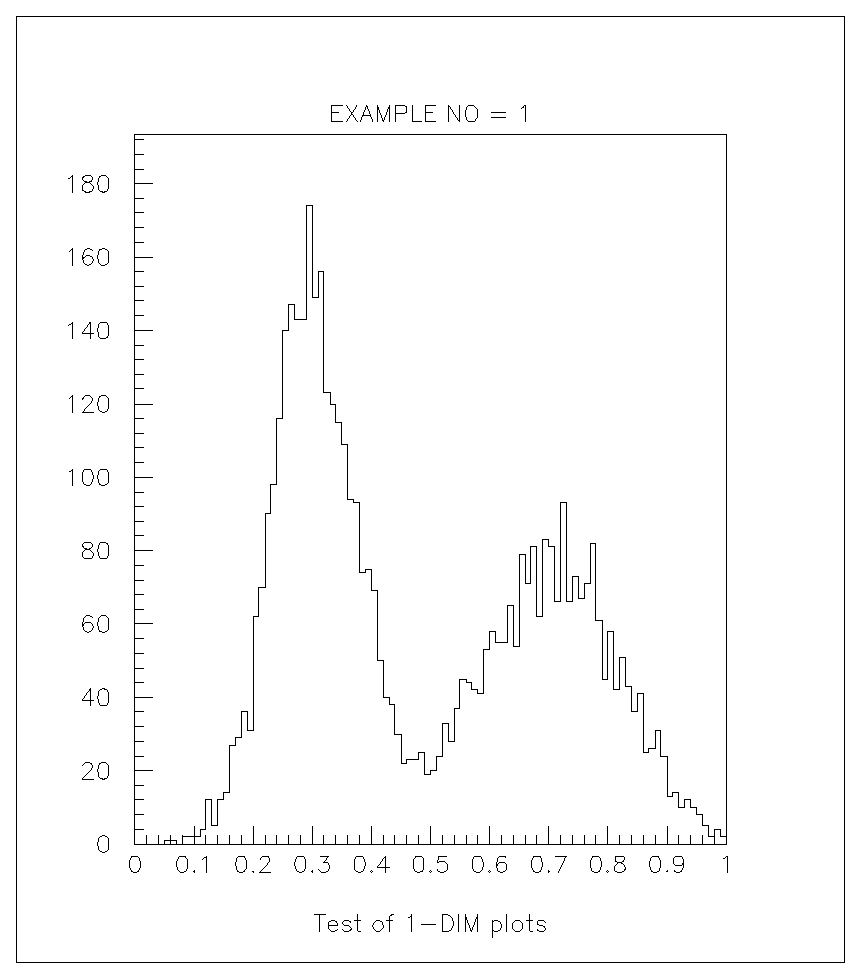
\includegraphics{hplot11.eps}\end{center}
\end{Fighere}
\begin{Fighere}
\begin{center}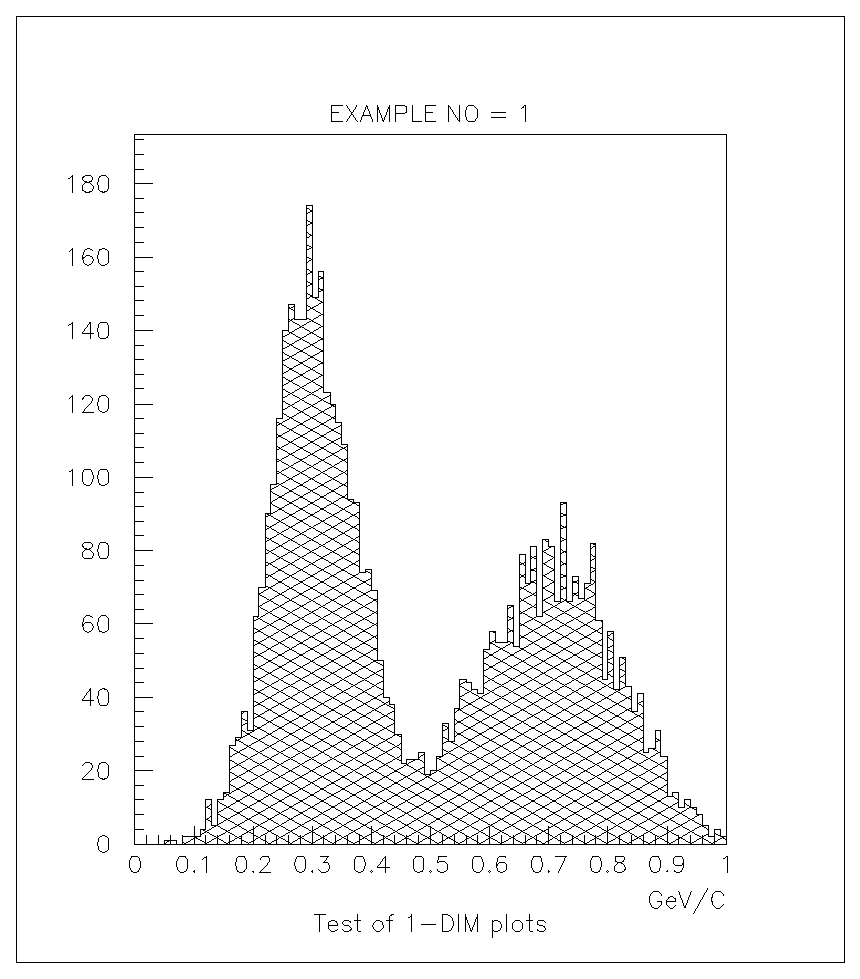
\includegraphics{hplot12.eps}\end{center}
\end{Fighere}
\begin{Fighere}
\begin{center}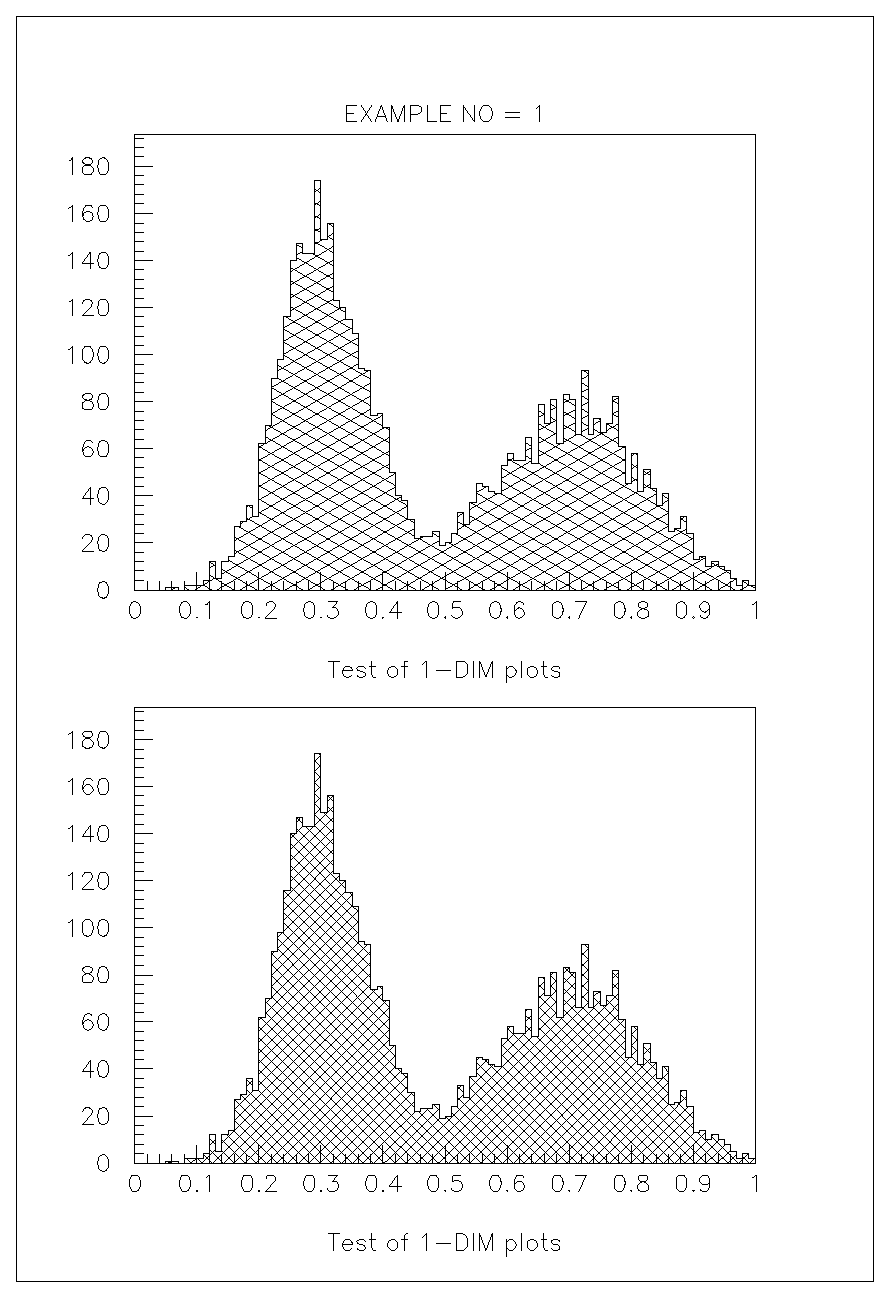
\includegraphics{hplot13.eps}\end{center}
\end{Fighere}


\newpage

\begin{XMPt}{Examples of basic HPLOT : 2-DIM histograms}
      SUBROUTINE HPLEX2
*
      CALL HTITLE('EXAMPLE NO = 2')
*
      CALL HPLSIZ(14.,14.,' ')
      CALL HPLSET('YGTI',0.3)
      CALL HPLSET('XMGL',1.)
      CALL HPLSET('YMGL',1.)
      CALL HPLSET('XMGR',1.)
      CALL HPLSET('YMGU',1.)
      CALL HPLSET('VSIZ',0.2)
      CALL HPLSET('YHTI',0.6)
      CALL IGSET('MTYP',1.)
      CALL HPLOT(200,' ',' ',0)
      CALL HPLCON(200,10,1)
      CALL HPLEGO(200,30.,30.)
      CALL HPLSUR(200,30.,30.,1)
*
      END
\end{XMPt}
\newpage
\begin{Fighere}
\begin{center}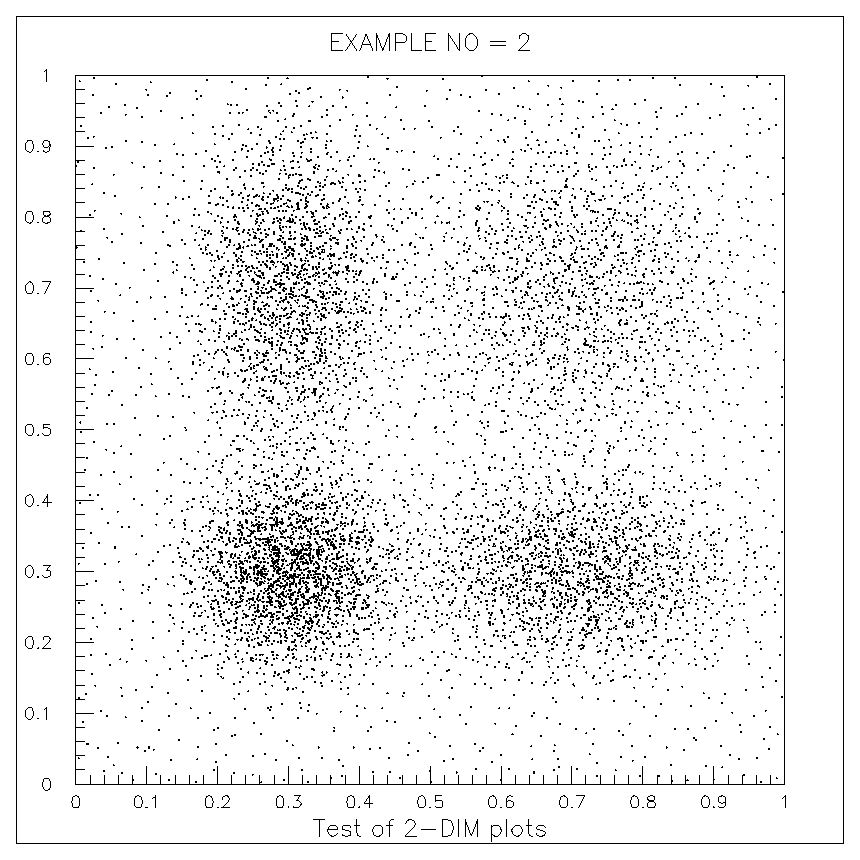
\includegraphics{hplot21.eps}\end{center}
\end{Fighere}
\begin{Fighere}
\begin{center}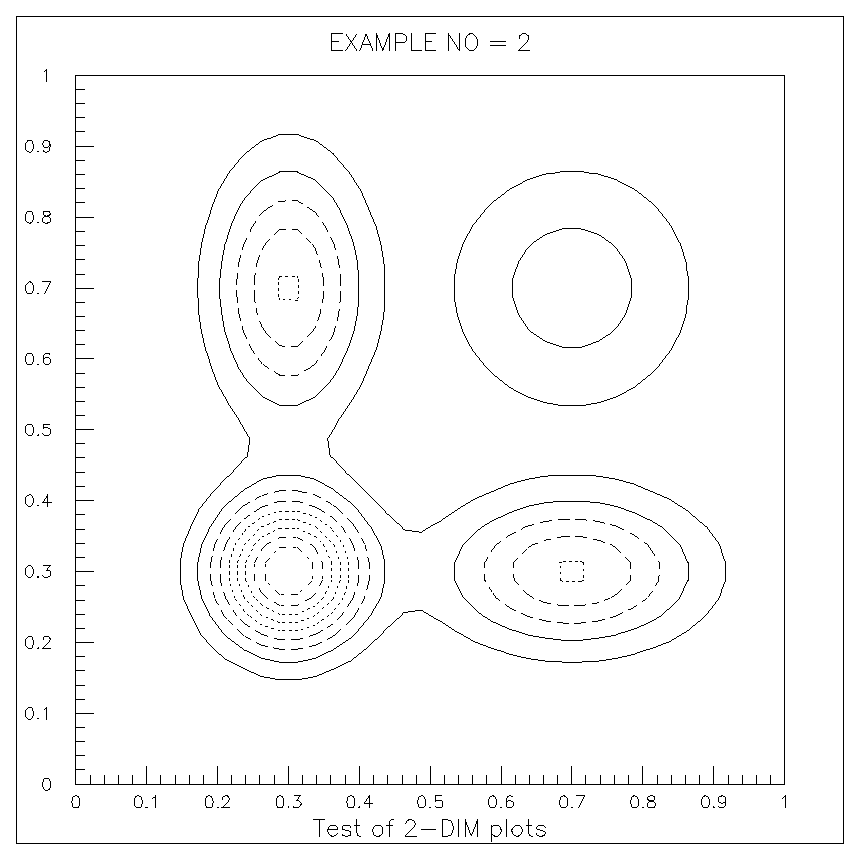
\includegraphics{hplot22.eps}\end{center}
\end{Fighere}
\begin{Fighere}
\begin{center}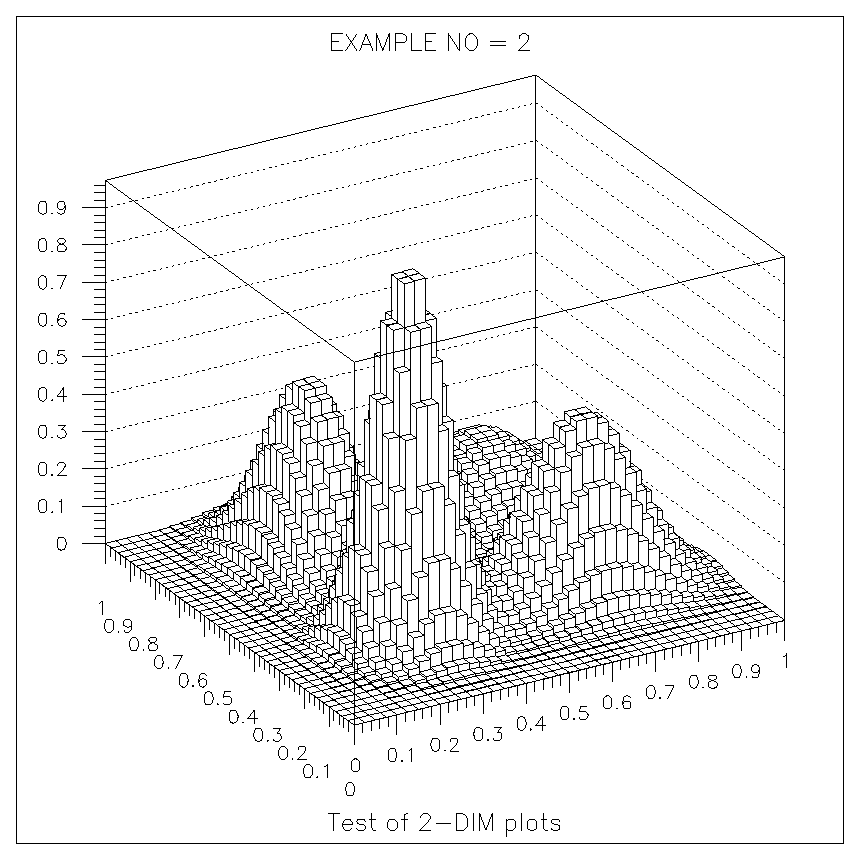
\includegraphics{hplot23.eps}\end{center}
\end{Fighere}
\begin{Fighere}
\begin{center}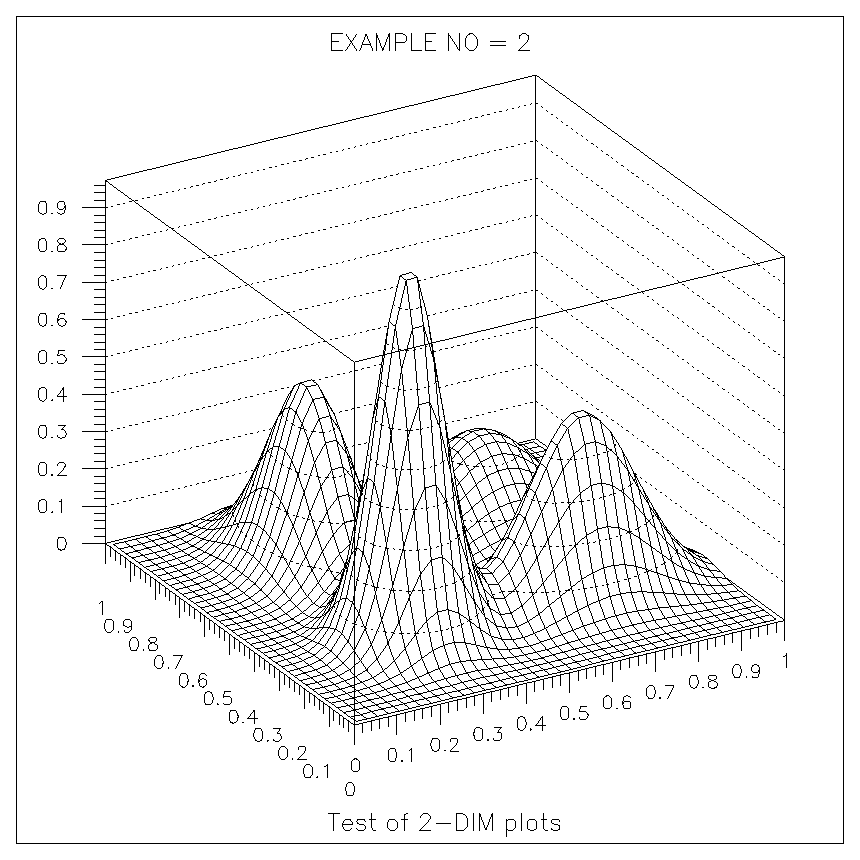
\includegraphics{hplot24.eps}\end{center}
\end{Fighere}

\newpage

\begin{XMPt}{Examples of HPLOT options}
      SUBROUTINE HPLEX3
*
      CALL HTITLE('EXAMPLE NO = 3')
*
      CALL HPLSIZ(14.5,20.,' ')
      CALL HPLSET('GSIZ',0.5)
      CALL HOPERA(110,'+',110,120,0.5,0.)
      CALL HOPERA(120,'+',120,130,0.5,0.)
      CALL HPLSET('PASS',5.)
      CALL HPLSET('CSHI',0.03)
      CALL HPLSET('XVAL',0.15)
      CALL HPLOPT('TIC ',1)
      CALL HPLOT(110,' ',' ',0)
      CALL HPLSET('HTYP',245.)
      CALL HPLOT(120,'S',' ',0)
      CALL HPLSET('HTYP',254.)
      CALL HPLOT(130,'S',' ',0)
      CALL HPLSOF(7.,12.,'LEP4 Very Preliminary',0.5,45.,99.,-1)
*
      END
\end{XMPt}
\newpage
\begin{Fighere}
\begin{center}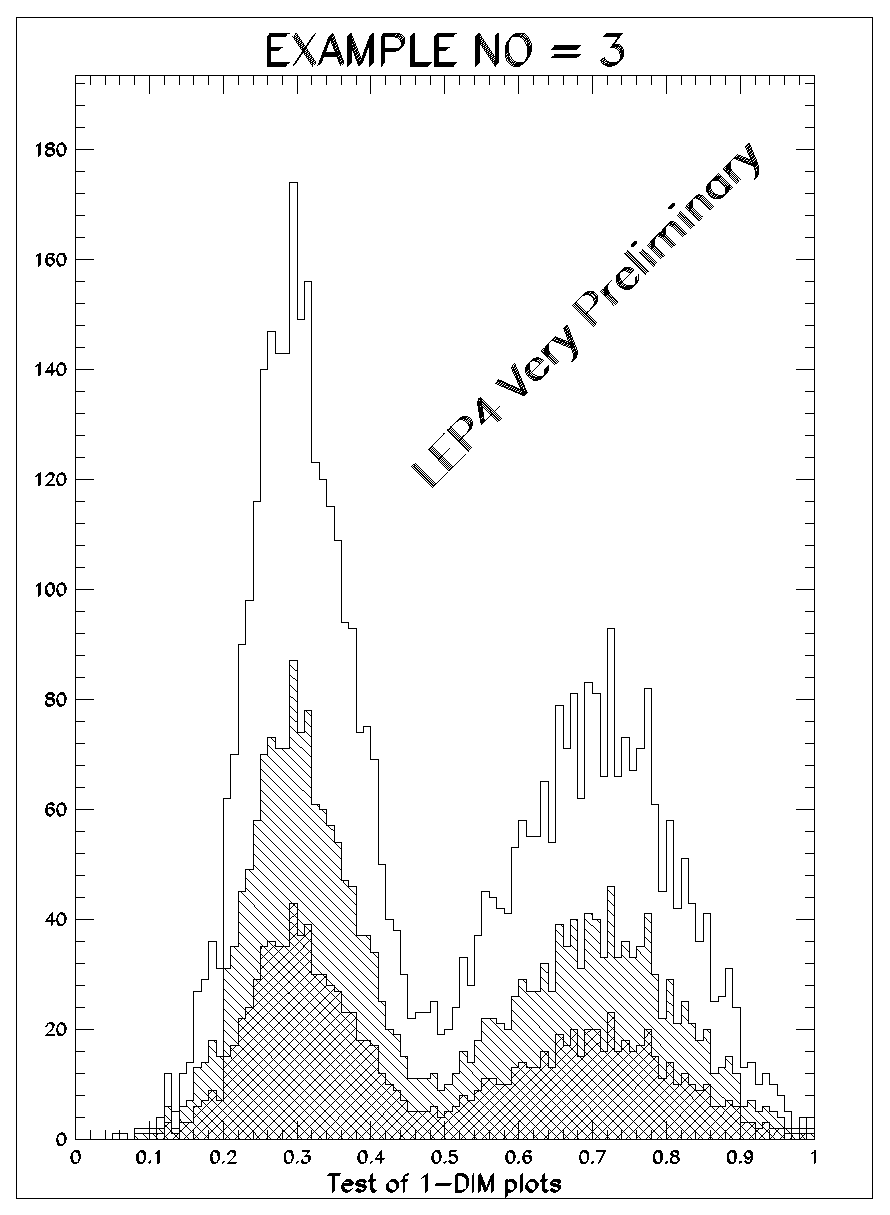
\includegraphics{hplot31.eps}\end{center}
\end{Fighere}

\newpage

\begin{XMPt}{ Examples of HPLOT options}
      SUBROUTINE HPLEX4
*
      DIMENSION X(100),Y(100),EX(100),EY(100)
*
      CALL HTITLE('EXAMPLE NO = 4')
*
      CALL HCOPY(110,310,' ')
      CALL HRESET(310,' ')
      CALL HPLSET('XMGL',1.)
      CALL HPLSET('YMGL',1.)
      CALL HPLSET('XMGR',1.)
      CALL HPLSET('YMGU',1.)
      CALL HPLSET('VSIZ',0.2)
      CALL HPLSET('XVAL',0.15)
      CALL HPLSET('YGTI',0.3)
      CALL HPLSET('YHTI',0.6)
      CALL HPLSIZ(14.5,21.,' ')
      CALL HPLZON(1,2,1,' ')
      CALL HMAXIM(310,200.)
      CALL HMINIM(310,-25.)
      CALL HPLOT(310,' ',' ',0)
      CALL HREBIN(110,X,Y,EX,EY,50,1,100)
      CALL HPLERR(X,Y,EX,EY,48,' ',25,0.15)
      CALL HPLKEY(9.,18.,25,'p,K^+!,K^-!,[S,W')
*
      CALL HPLOT(310,' ',' ',0)
      CALL HREBIN(110,X,Y,EX,EY,20,1,100)
      CALL HPLERR(X,Y,EX,EY,20,' ',22,0.2)
      CALL HPLKEY(9.,8.,22,'[p^+!,p^-!,m^+!,m^-')
      CALL HDELET(120)
      CALL HDELET(130)
      CALL HDELET(310)
*
      END
\end{XMPt}
\newpage
\begin{Fighere}
\begin{center}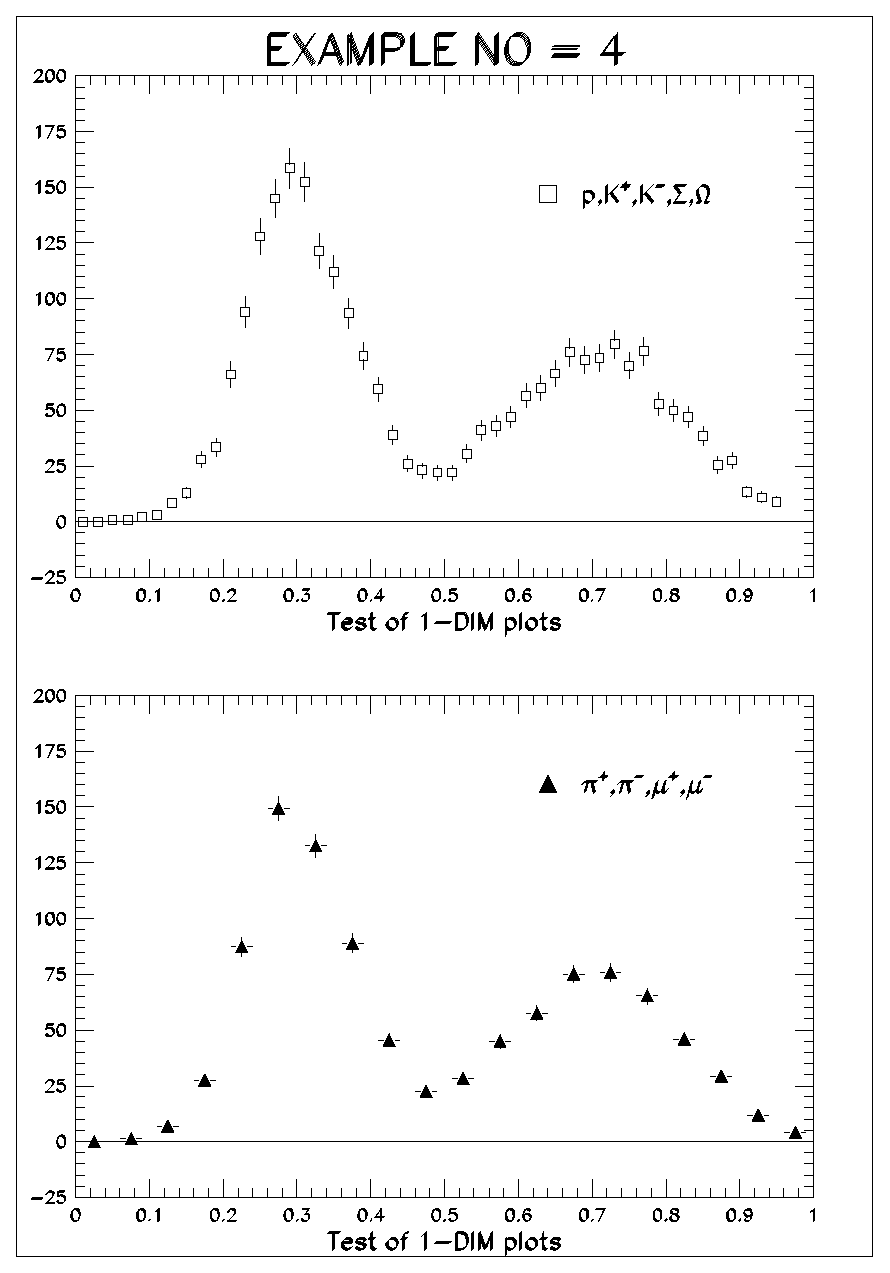
\includegraphics{hplot41.eps}\end{center}
\end{Fighere}

\newpage

\begin{XMPt}{Examples of HPLOT options (BARS)}
      SUBROUTINE HPLEX5
*
      DIMENSION XALL(12),XFEM(12)
      DATA XALL/
     +100.,200.,300.,500.,400.,700.,600.,400.,500.,300.,200.,100./
      DATA XFEM/
     + 70.,220.,330.,480.,440.,650.,300.,100.,200.,300.,200.,300./
*
      CALL HTITLE('EXAMPLE NO = 5')
*
      CALL HPLSET('YGTI',0.3)
      CALL HPLSIZ(14.5,21.,' ')
      CALL HPLZON(1,2,1,' ')
      CALL HBOOK1(1,'Distribution of grades (males)',12,2.,14.,0.)
      CALL HPAK(1,XALL)
      CALL HPLOPT('BAR ',1)
      CALL HPLSET('HTYP',188.)
      CALL HPLOT(1,' ',' ',0)
      CALL HRESET(1,'(Males and Females)')
      CALL HPAK(1,XALL)
      CALL HPLSET('BARO',0.)
      CALL HPLSET('BARW',0.3)
      CALL HPLOT(1,' ',' ',0)
      CALL HPLSET('HTYP',211.)
      CALL HPLSET('BARO',0.4)
      CALL HPAK(1,XFEM)
      CALL HPLOT(1,'SAME',' ',0)
      CALL HPLOPT('NBAR',1)
      CALL HDELET(1)
      CALL HPLSET('*',0.)
*
      END
\end{XMPt}
\newpage
\begin{Fighere}
\begin{center}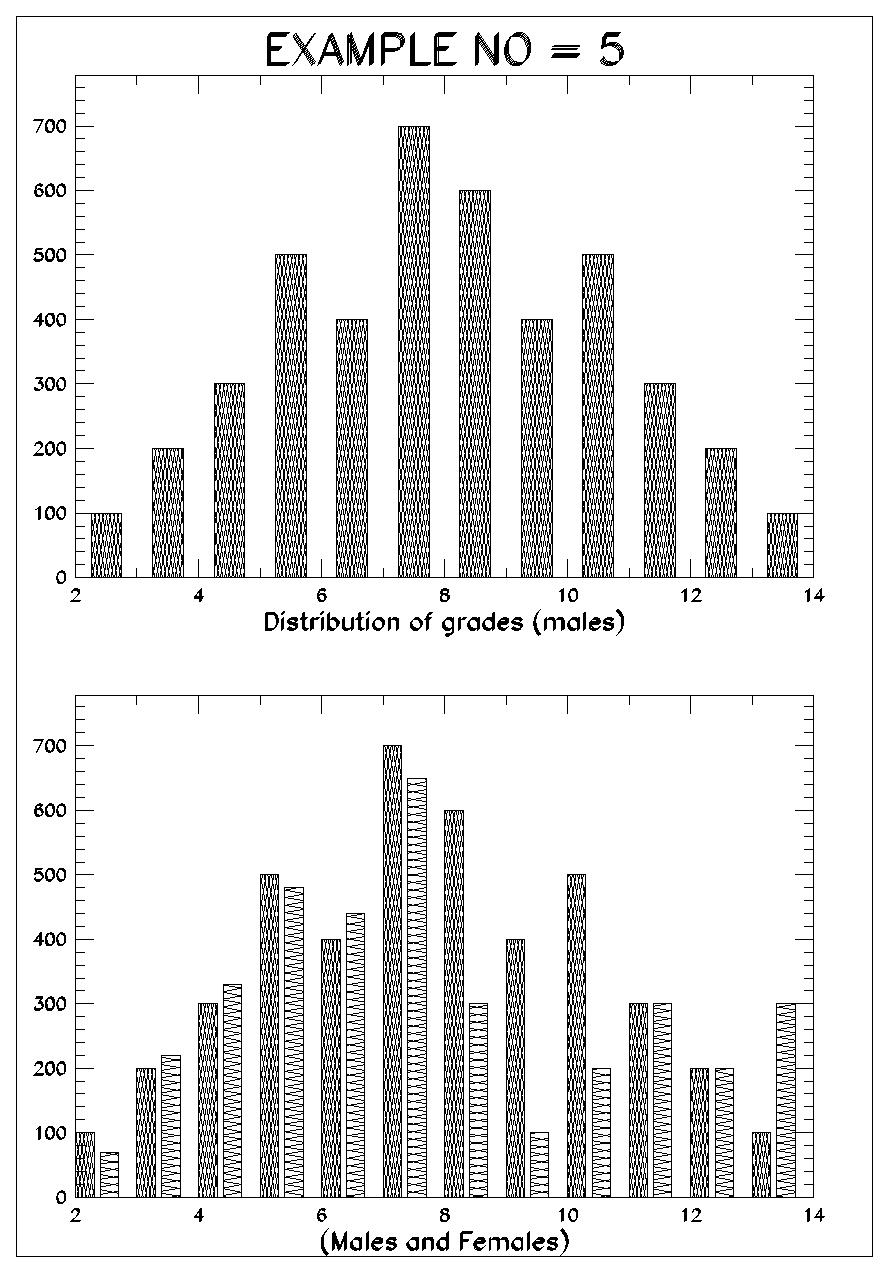
\includegraphics{hplot51.eps}\end{center}
\end{Fighere}

\newpage

\begin{XMPt}{Examples of HPLOT using GKS metafiles or HIGZ files}
      SUBROUTINE HPLEX6
*
      CALL HPLEX1
      CALL HPLEX2
      CALL HPLEX3
      CALL HPLEX4
      CALL HPLEX5
      CALL HPLNUL
*
      END
\end{XMPt}

\begin{XMPt}{Examples of HPLOT playing back HIGZ files}
      SUBROUTINE HPLEX7
*
      CHARACTER*10 STR
      DATA ICYCLE/999/
*
      CALL RZLDIR(' ',' ')
      CALL IGSET('AURZ',0.)
      CALL IZIN('PICT1',ICYCLE)
      CALL IZPICT('PICT1','D')
      CALL IRQST(1,1,ISTAT,NCH,STR)
      CALL IZIN('PICT8',ICYCLE)
      CALL IZPICT('PICT8','D')
      CALL IRQST(1,1,ISTAT,NCH,STR)
      CALL IZIN('PICT9',ICYCLE)
      CALL IZPICT('PICT9','D')
      CALL IRQST(1,1,ISTAT,NCH,STR)
*
      END
\end{XMPt}
